% =====================================================================
% Anexo D: prueba simulada del Modulo 4 (movida desde el capitulo 3
% cuando el Modulo 4 real se ejecuto con la escena de control).
% =====================================================================

\section*{Anexo D. Prueba simulada del Módulo 4}
\label{sec:m4-simulado}
\phantomsection\addcontentsline{toc}{section}{Anexo D. Prueba simulada del Módulo 4}

% Numeracion propia del anexo: figuras y tablas como D.n
\setcounter{figure}{0}\renewcommand{\thefigure}{D.\arabic{figure}}
\setcounter{table}{0}\renewcommand{\thetable}{D.\arabic{table}}

Esta prueba se diseñó antes de contar con el entrenamiento de ArCH y con la
ejecución real del Módulo~4 (Sección~\ref{sec:res-unidad3}); se conserva como
anexo porque explica, con descriptores de calidad controlada, de qué depende el
comportamiento de la fusión. Los descriptores de los Módulos~2 y~3 se inventan
sobre una escena sintética en la que se conoce la clase de cada punto. El
programa es \texttt{simular\_modulo4.py}, en la carpeta
\texttt{experimentacion/modulo4\_simulado} del repositorio, y corre en el equipo
local en unos tres minutos, sin GPU.

La prueba tiene dos límites. No entrena ninguna red, porque los descriptores
están fijos y los prototipos se refinan alternando asignación y promedio, que es
lo que haría el ciclo de entrenamiento con descriptores fijos. Y no predice el
mIoU de la Catedral, porque los descriptores son inventados. Lo que muestra es
cómo se comporta el Módulo~4 y de qué depende.

\paragraph*{Escena.}
La escena es una nave de 20 por 10\,m con 23\,600 puntos. Las clases conocidas
son el suelo y los muros, con 12\,000 puntos. Las clases nuevas son la columna,
el pilar y la bóveda, con 11\,600 puntos. Columna y pilar tienen la misma forma,
un cilindro de 0{,}3\,m de radio y 6\,m de alto, y están intercalados en la nave,
de modo que ni la geometría ni la posición los distinguen. Es el caso que motiva
este trabajo, separar elementos que se parecen en forma pero no en significado.

\paragraph*{Descriptores.}
Cada descriptor es el centro de su clase más un desvío propio de cada objeto y
un ruido por punto. El desvío por objeto representa que cada columna concreta se
aparta de su clase, y no se cancela al promediar los puntos de una región. El
descriptor $f_{\mathrm{sem}}$, de 96 dimensiones, separa bien las clases
conocidas y apenas las nuevas, porque la red solo vio etiquetas de las conocidas.
El descriptor $f_{\mathrm{ssl}}$, de 1088 dimensiones, separa las clases nuevas
con una fuerza que se controla y que hace de calidad de Sonata. El descriptor
$f_{\mathrm{geo}}$ de la línea base se calcula con la fórmula de la
Sección~\ref{sec:fgeo}. Salvo que se indique otra cosa, la calidad de Sonata es
1{,}5, un valor intermedio, $\alpha=0{,}5$ y $M=8$.

\subsubsection*{Paso 1. Concatenación}

Cada punto de una clase nueva recibe su descriptor $F_i$, la concatenación de
$f_{\mathrm{sem}}$ con $f_{\mathrm{geo}}$ en la línea base o con
$f_{\mathrm{ssl}}$ en la propuesta, según la Ec.~\eqref{eq:hibrido}. Antes de
concatenar, cada parte se lleva a largo 1, para que la de 1088 dimensiones no
domine a la de 96 solo por tener más números.

\begin{algorithm}[H]
\small
\caption{Paso 1 del Módulo~4, concatenación.}
\KwIn{$f_{\mathrm{sem}}$ y $f_x$ de cada punto nuevo, con $f_x$ igual a $f_{\mathrm{geo}}$ o a $f_{\mathrm{ssl}}$}
\KwOut{descriptor $F_i$ de cada punto}
\ForEach{punto $i$ de una clase nueva}{
  $F_i \leftarrow [\,f_{\mathrm{sem}}(i)/\lVert f_{\mathrm{sem}}(i)\rVert \mid f_x(i)/\lVert f_x(i)\rVert\,]$\;
}
\end{algorithm}

\subsubsection*{Paso 2. Regiones}

Los puntos de las clases nuevas se agrupan con DBSCAN, con radio de 0{,}5\,m,
según la Sección~\ref{sec:region}, y el descriptor de cada región es el promedio
de los de sus puntos. En la escena salen 12 regiones, cuatro por clase, una por
columna, una por pilar y una por tramo de bóveda. La Figura~\ref{fig:m4-regiones}
las muestra.

\begin{algorithm}[H]
\small
\caption{Paso 2 del Módulo~4, regiones.}
\KwIn{coordenadas y $F_i$ de los puntos nuevos, radio $0{,}5$\,m}
\KwOut{regiones $r$, su descriptor $F^{(r)}$ y su rasgo geométrico $g^{(r)}$}
regiones $\leftarrow$ DBSCAN sobre las coordenadas\;
\ForEach{región $r$}{
  $F^{(r)} \leftarrow$ promedio de $F_i$ de sus puntos\;
  $g^{(r)} \leftarrow$ linealidad, planaridad, dispersión y centroide de sus puntos\;
}
\end{algorithm}

\begin{figure}[!htbp]
\centering
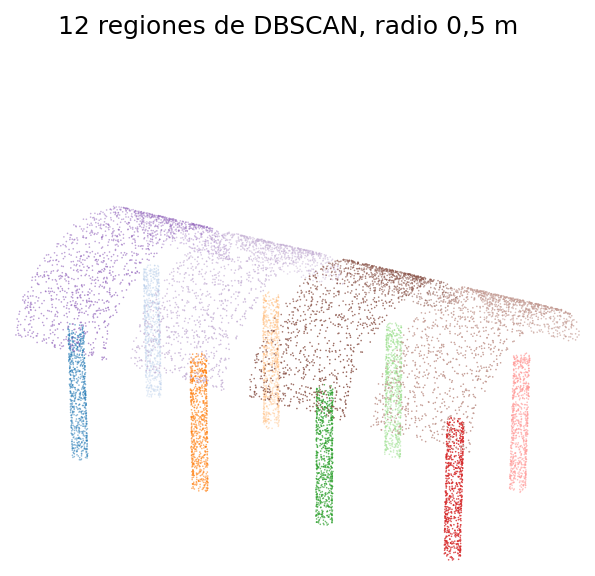
\includegraphics[width=0.55\linewidth]{imagenes/m4_paso2_regiones.png}
\caption[Regiones de la escena simulada]{Regiones de la escena simulada, una por color. Elaboración propia.}
\label{fig:m4-regiones}
\end{figure}

\subsubsection*{Paso 3. Afinidad entre regiones}

Para cada par de regiones se calculan dos afinidades, que van de 0, nada
parecidas, a 1, iguales. La afinidad geométrica $S_g$, según la
Ec.~\eqref{eq:gauss}, responde a si se parecen en forma y en posición, y usa solo
$g$. La afinidad semántica $S_s$, según la Ec.~\eqref{eq:afinidad}, responde a si
se parecen en lo que son, y usa el descriptor $F$, por donde entra Sonata. Las dos
se combinan en $S_b=\alpha S_g+(1-\alpha)S_s$, según la Ec.~\eqref{eq:afinidad}.

La Figura~\ref{fig:m4-afinidad} muestra las tres matrices, con las regiones
ordenadas por clase. $S_g$ separa la bóveda del resto, pero no columna de pilar,
porque tienen la misma forma. $S_s$ de la línea base es alta en casi todas las
parejas, es decir, todo se parece a todo. $S_s$ de la propuesta muestra tres
bloques en la diagonal, de modo que las regiones de una misma clase se parecen
entre sí y poco a las demás. La Tabla~\ref{tab:m4-caso} lo concreta con una
columna, un pilar y un tramo de bóveda. La línea base dice que la columna se
parece más a la bóveda, 0{,}94, que al pilar, 0{,}79, y por eso confunde parte de
la bóveda con el pilar.

\begin{figure}[!htbp]
\centering\setstretch{1}
\begin{tikzpicture}[font=\scriptsize, node distance=4mm]
\node[fdato] (a) {Descriptores $F^{(r)}$ y rasgos $g^{(r)}$ de las 12 regiones};
\node[fop, below=of a] (b) {$S_s\leftarrow$ coseno entre cada par de descriptores};
\node[fop, below=of b] (c) {$S_g\leftarrow$ núcleo gaussiano entre cada par de rasgos};
\node[fop, below=of c] (d) {$S_b\leftarrow\alpha S_g+(1-\alpha)S_s$, con $\alpha=0{,}5$};
\node[fdato, below=of d] (e) {Matriz $S_b$ de $12\times 12$};
\foreach \u/\v in {a/b,b/c,c/d,d/e} \draw[ffl] (\u) -- (\v);
\end{tikzpicture}
\caption[Afinidad entre regiones]{Afinidad entre regiones. Elaboración propia.}
\end{figure}

\begin{figure}[!htbp]
\centering
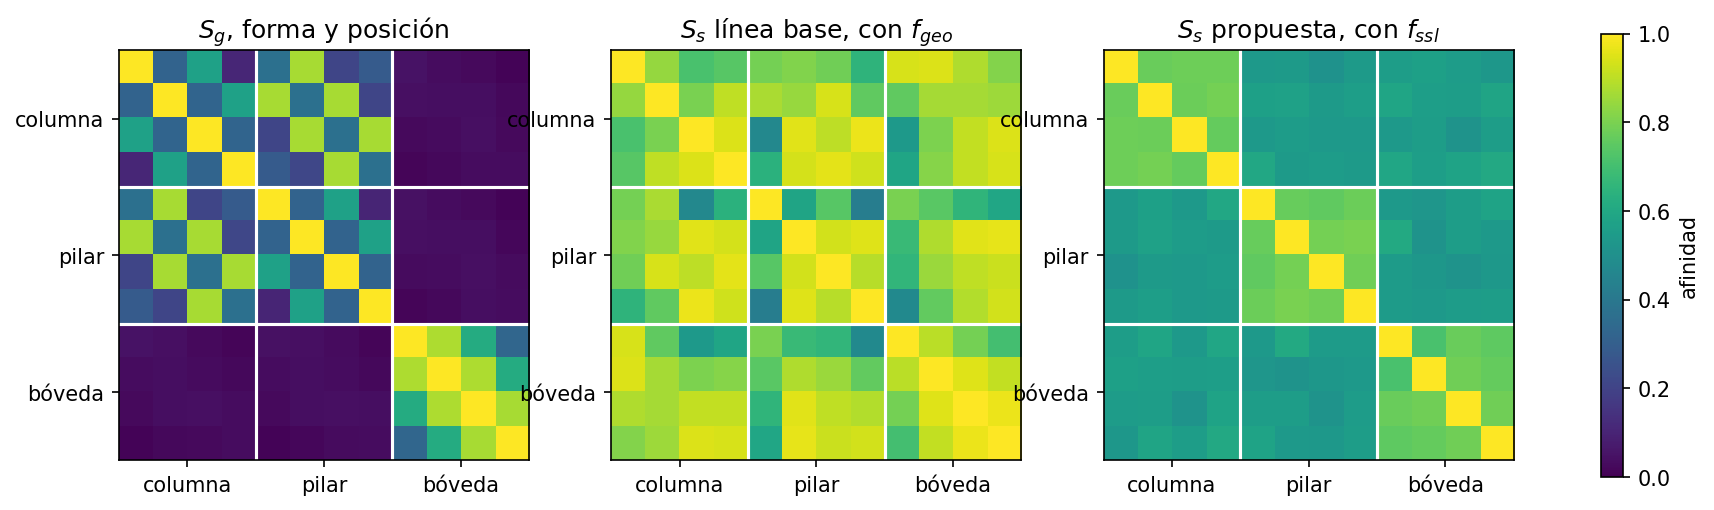
\includegraphics[width=\linewidth]{imagenes/m4_paso3_afinidad.png}
\caption[Matrices de afinidad de la escena simulada]{Matrices de afinidad de la escena simulada, con las regiones ordenadas por clase. Elaboración propia.}
\label{fig:m4-afinidad}
\end{figure}

\begin{table}[!htbp]
\centering
\setstretch{1}\small
\caption[Afinidades de una columna con un pilar y con la bóveda]{Afinidades de una columna con un pilar y con un tramo de bóveda en la escena simulada. Elaboración propia.}
\label{tab:m4-caso}
\begin{tabularx}{\linewidth}{@{}>{\raggedright\arraybackslash}X ccc@{}}
\toprule
\textbf{Par de regiones} & \textbf{$S_g$} & \textbf{$S_s$ línea base} & \textbf{$S_s$ propuesta} \\
\midrule
Columna y pilar, misma forma & 0{,}37 & 0{,}79 & 0{,}54 \\
Columna y bóveda, distinta forma & 0{,}05 & 0{,}94 & 0{,}55 \\
\bottomrule
\end{tabularx}
\end{table}

$S_g$ entre columna y pilar vale 0{,}37 y no 1, aunque la forma sea la misma,
porque $g$ incluye el centroide y los dos están en lugares distintos. La
propuesta quita las dos similitudes falsas, pero en este par concreto no deja la
columna más cerca del pilar que de la bóveda. La mejora aparece al combinar todas
las regiones en el hipergrafo, que es lo que hacen los pasos siguientes.

\subsubsection*{Paso 4. Hiperaristas}

Cada región forma una hiperarista con sus $M=8$ regiones más afines según $S_b$,
como se explica en la Sección~\ref{sec:hiperarista}. Su descriptor pasa a ser el
promedio de los de su hiperarista, ponderado por la afinidad. Así una región
toma información de las que se le parecen. La Figura~\ref{fig:m4-hiperarista}
muestra la hiperarista de una columna. En la escena solo hay otras tres columnas.
La propuesta las incluye a las tres entre sus ocho vecinos, y la línea base solo a
dos.

\begin{algorithm}[H]
\small
\caption{Paso 4 del Módulo~4, hiperaristas.}
\KwIn{descriptores $F^{(r)}$, matriz $S_b$, $M=8$}
\KwOut{descriptor enriquecido $\hat{F}^{(r)}$ de cada región}
\ForEach{región $r$}{
  $e_r \leftarrow r$ y sus $M$ regiones con mayor $S_b$\;
  $\hat{F}^{(r)} \leftarrow$ promedio de $F$ en $e_r$, ponderado por $S_b$\;
}
\end{algorithm}

\begin{figure}[!htbp]
\centering
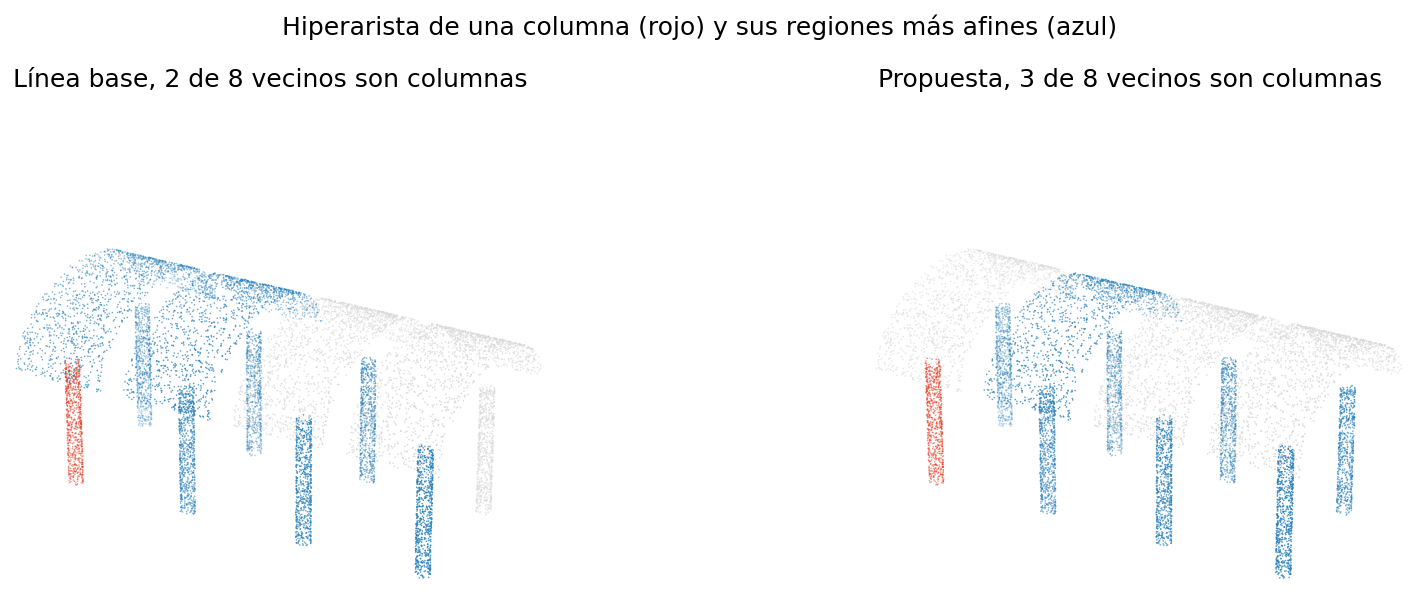
\includegraphics[width=\linewidth]{imagenes/m4_paso4_hiperarista.png}
\caption[Hiperarista de una columna en las dos versiones]{Hiperarista de una columna en la línea base y en la propuesta. Elaboración propia.}
\label{fig:m4-hiperarista}
\end{figure}

\subsubsection*{Paso 5. Prototipos y pseudo-etiquetas}

Se forman tres prototipos, uno por clase nueva. Cada región se compara con ellos
y la normalización de Sinkhorn-Knopp, según la Sección~\ref{sec:sinkhorn},
convierte esas comparaciones en un reparto equilibrado entre las tres clases.
Cada prototipo se recalcula como el promedio de las regiones, ponderado por ese
reparto, según la Ec.~\eqref{eq:prototipo}, y el ciclo se repite quince veces.
Sinkhorn equilibra puntos y no regiones, como dice la Sección~\ref{sec:sinkhorn},
así que cada región pesa tanto como puntos tiene. Al final, cada región toma la
clase con mayor reparto, y sus puntos la heredan.

\begin{figure}[!htbp]
\centering\setstretch{1}
\begin{tikzpicture}[font=\scriptsize, node distance=4mm]
\node[fdato] (a) {Descriptores enriquecidos $\hat{F}^{(r)}$ de las 12 regiones};
\node[fop, below=of a] (b) {Tres prototipos iniciales, elegidos lejos entre sí};
\node[fop, below=of b] (c) {Comparar cada región con cada prototipo};
\node[fop, below=of c] (d) {Sinkhorn, reparto equilibrado por puntos};
\node[fop, below=of d] (e) {Recalcular cada prototipo con ese reparto};
\node[fdec, below=of e] (f) {¿15 vueltas?};
\node[fdato, below=of f] (g) {Clase de cada región y de sus puntos};
\foreach \u/\v in {a/b,b/c,c/d,d/e,e/f} \draw[ffl] (\u) -- (\v);
\draw[ffl] (f) -- node[left, font=\tiny]{sí} (g);
\draw[ffl] (f.east) -- node[above, font=\tiny]{no} ++(1.2,0) |- (c.east);
\end{tikzpicture}
\caption[Prototipos y pseudo-etiquetas]{Prototipos y pseudo-etiquetas. Elaboración propia.}
\end{figure}

La Figura~\ref{fig:m4-escena} muestra el resultado de una repetición. La línea
base confunde la mitad de la bóveda con el pilar y no separa columnas de pilares.
La propuesta asigna bien las tres clases en esa repetición. El promedio de cinco
repeticiones, con la calidad de Sonata en 1{,}5, es un mIoU de las clases nuevas
de 0{,}35 en la línea base y de 0{,}75 en la propuesta.

\begin{figure}[!htbp]
\centering
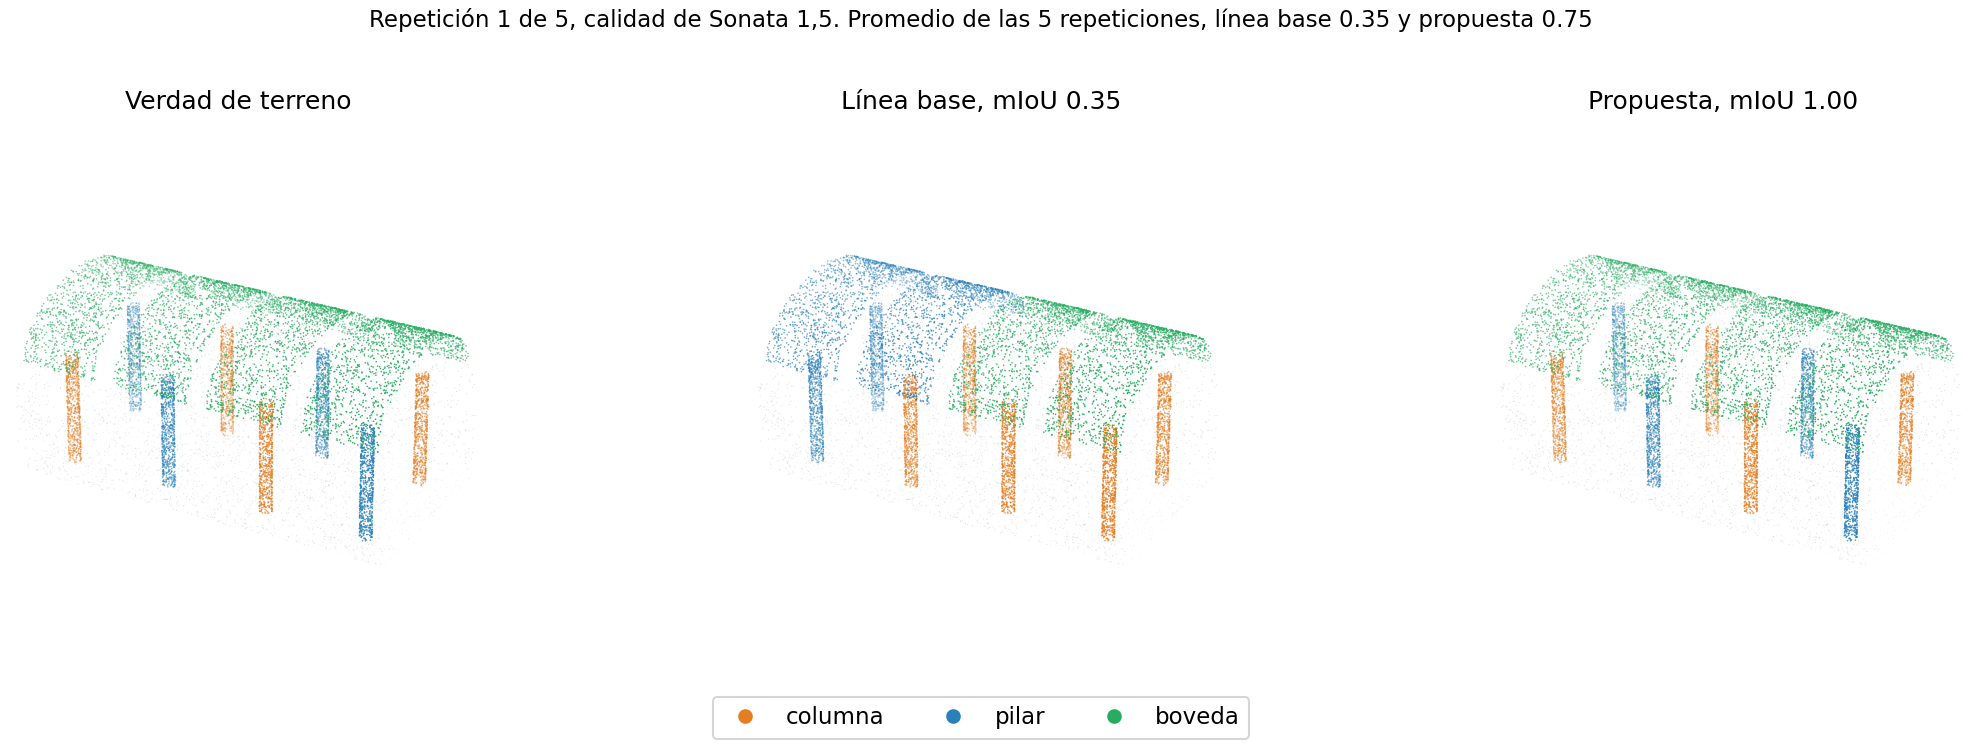
\includegraphics[width=\linewidth]{imagenes/m4_paso5_escena.png}
\caption[Resultado del Módulo 4 simulado]{Verdad de terreno, línea base y propuesta en una repetición de la escena simulada. Elaboración propia.}
\label{fig:m4-escena}
\end{figure}

\subsubsection*{De qué depende el resultado}

Se repitió la prueba variando un parámetro cada vez, con cinco repeticiones por
valor. La métrica es el mIoU de las tres clases nuevas, con un emparejamiento
húngaro porque las clases descubiertas no tienen nombre. La
Figura~\ref{fig:m4-curvas} muestra los cinco barridos y la
Tabla~\ref{tab:m4-escenarios} los resume.

\begin{figure}[!htbp]
\centering
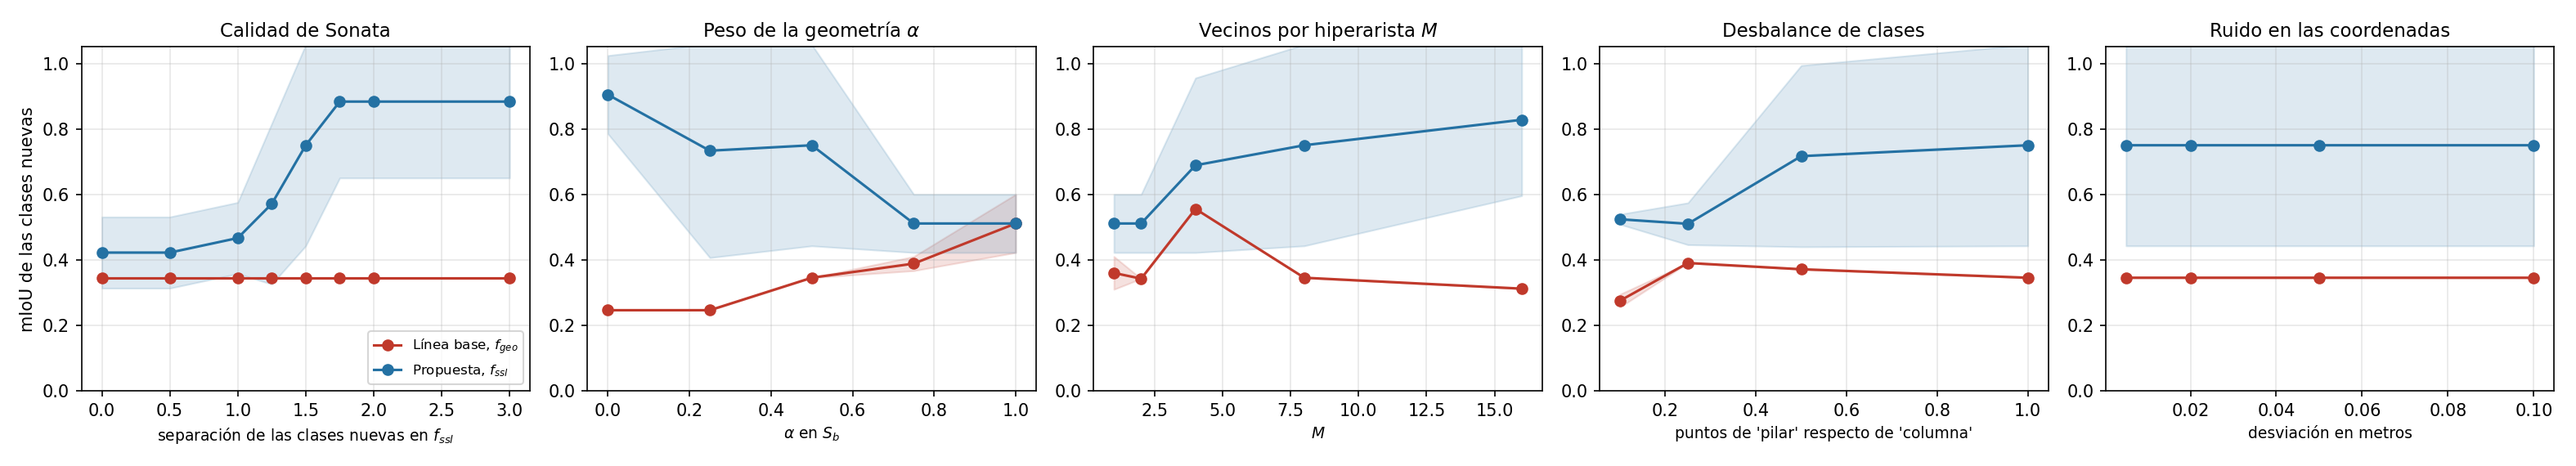
\includegraphics[width=\linewidth]{imagenes/m4_curvas.png}
\caption[Comportamiento del Módulo 4 simulado]{mIoU de las clases nuevas de la línea base y de la propuesta en cada barrido. La banda es la desviación entre repeticiones. Elaboración propia.}
\label{fig:m4-curvas}
\end{figure}

\begin{table}[!htbp]
\centering
\setstretch{1}\small
\caption[Resultados de la prueba simulada del Módulo 4]{Resultados de la prueba simulada del Módulo 4. Elaboración propia.}
\label{tab:m4-escenarios}
\begin{tabularx}{\linewidth}{@{}>{\raggedright\arraybackslash\hsize=0.7\hsize}X>{\raggedright\arraybackslash\hsize=1.3\hsize}X@{}}
\toprule
\textbf{Barrido} & \textbf{Resultado} \\
\midrule
Calidad de Sonata, de 0 a 3 & La línea base queda en 0{,}35 siempre. La propuesta sube de 0{,}42 a 0{,}88. El aporte de $f_{\mathrm{ssl}}$ depende de que Sonata separe las clases nuevas \\
Peso de la geometría $\alpha$, de 0 a 1 & Con $\alpha=1$, solo geometría, las dos versiones dan 0{,}51, como debe ser. La propuesta mejora al bajar $\alpha$, porque lo que aporta está en $S_s$ \\
Vecinos por hiperarista $M$, de 1 a 16 & La propuesta mejora con $M$, de 0{,}51 a 0{,}83. Con 12 regiones, $M=16$ equivale a usarlas todas \\
Desbalance, pilar con el 100\,\% al 10\,\% de los puntos de la columna & La propuesta cae de 0{,}75 a 0{,}52. Sinkhorn reparte por igual y parte la clase grande cuando una clase es pequeña \\
Ruido en las coordenadas, de 0{,}5 a 10\,cm & Sin efecto, porque el radio de DBSCAN es mucho mayor \\
\bottomrule
\end{tabularx}
\end{table}

La variabilidad entre repeticiones es alta. Con solo 12 regiones, una región mal
asignada mueve mucho el mIoU, por eso las bandas de la Figura~\ref{fig:m4-curvas}
son anchas. Dos resultados orientan el trabajo con datos reales. El primero es que
el aporte de Sonata solo aparece cuando la forma no basta, que es justamente el
caso de la Catedral. El segundo es que el desbalance entre clases nuevas es un
modo de fallo del equilibrio de Sinkhorn, que habrá que vigilar con la tolerancia
$\gamma$ cuando una clase tenga pocos puntos.
